\chapter{Data Aquisition System\label{cha:chapter3}}
For labeled data acquisition a system was required that is able to function in a laboratory environment, as well as recieve the data coming from the field study. For this purpose TapSensing was created. TapSensing is an iOS application that collects touch events including their sensory information to then send them to a backend server application. In the following sections we will outline the different components of TapSensing. 

\section{System Architecture}
The TapSensing application comprises to two main components, one being the mobile application and the other being the server-side application. The mobile client is responsible for generating the sensor and tap information by providing a user interface for the user to tap. For the data to be stored in a centralized manner, the backend provides endpoints as a gateway to the database.

\begin{figure}[h!]
  \centering
  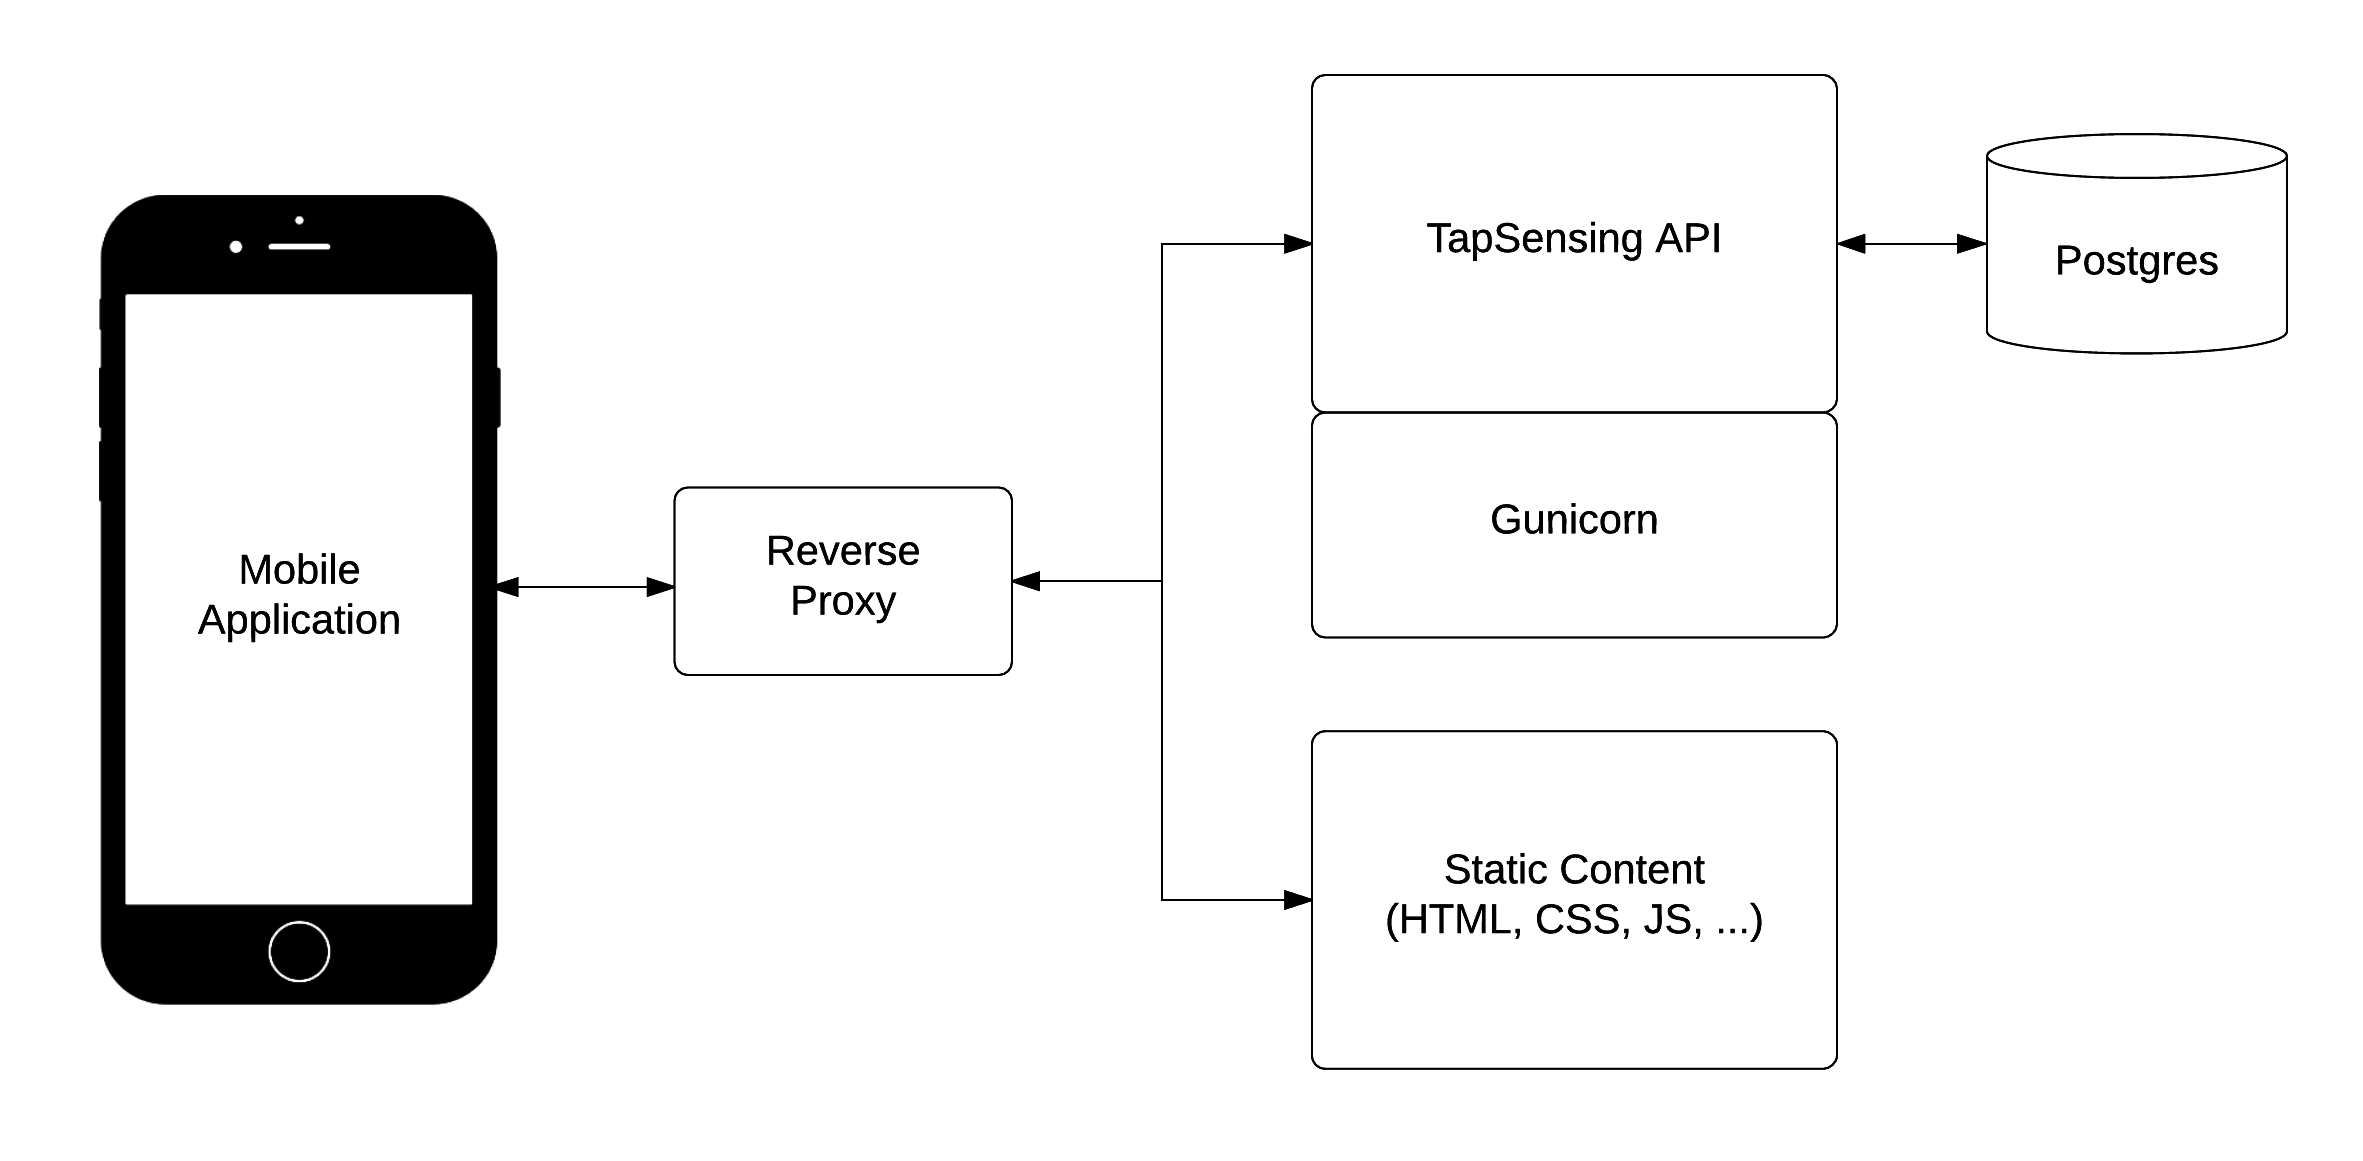
\includegraphics[width=1\textwidth]{tapsensing_architecutre_sw.png}
  \caption{TapSensing architecture overview.}
\end{figure}

For the network requests containing the tap information which come from the mobile device to reach the backend, it must first pass through a reverse proxy. As reverse proxy we have chosen NGINX due to it's easy configurability. In this case, NGINX forwards requests to the TapSensing application and serves static files.\\
The TapSensing backend is written upon the Python Django Framework\footnote{https://www.djangoproject.com/} which is being executed upon the gunicorn application server. Django uses a so-called ORM to perform transactions with the Database, which in our case is a PostgreSQL database.

\section{Mobile Application}
\subsection{Interface}
\subsubsection{Tap Input}

\begin{figure}[h!]
  \centering
  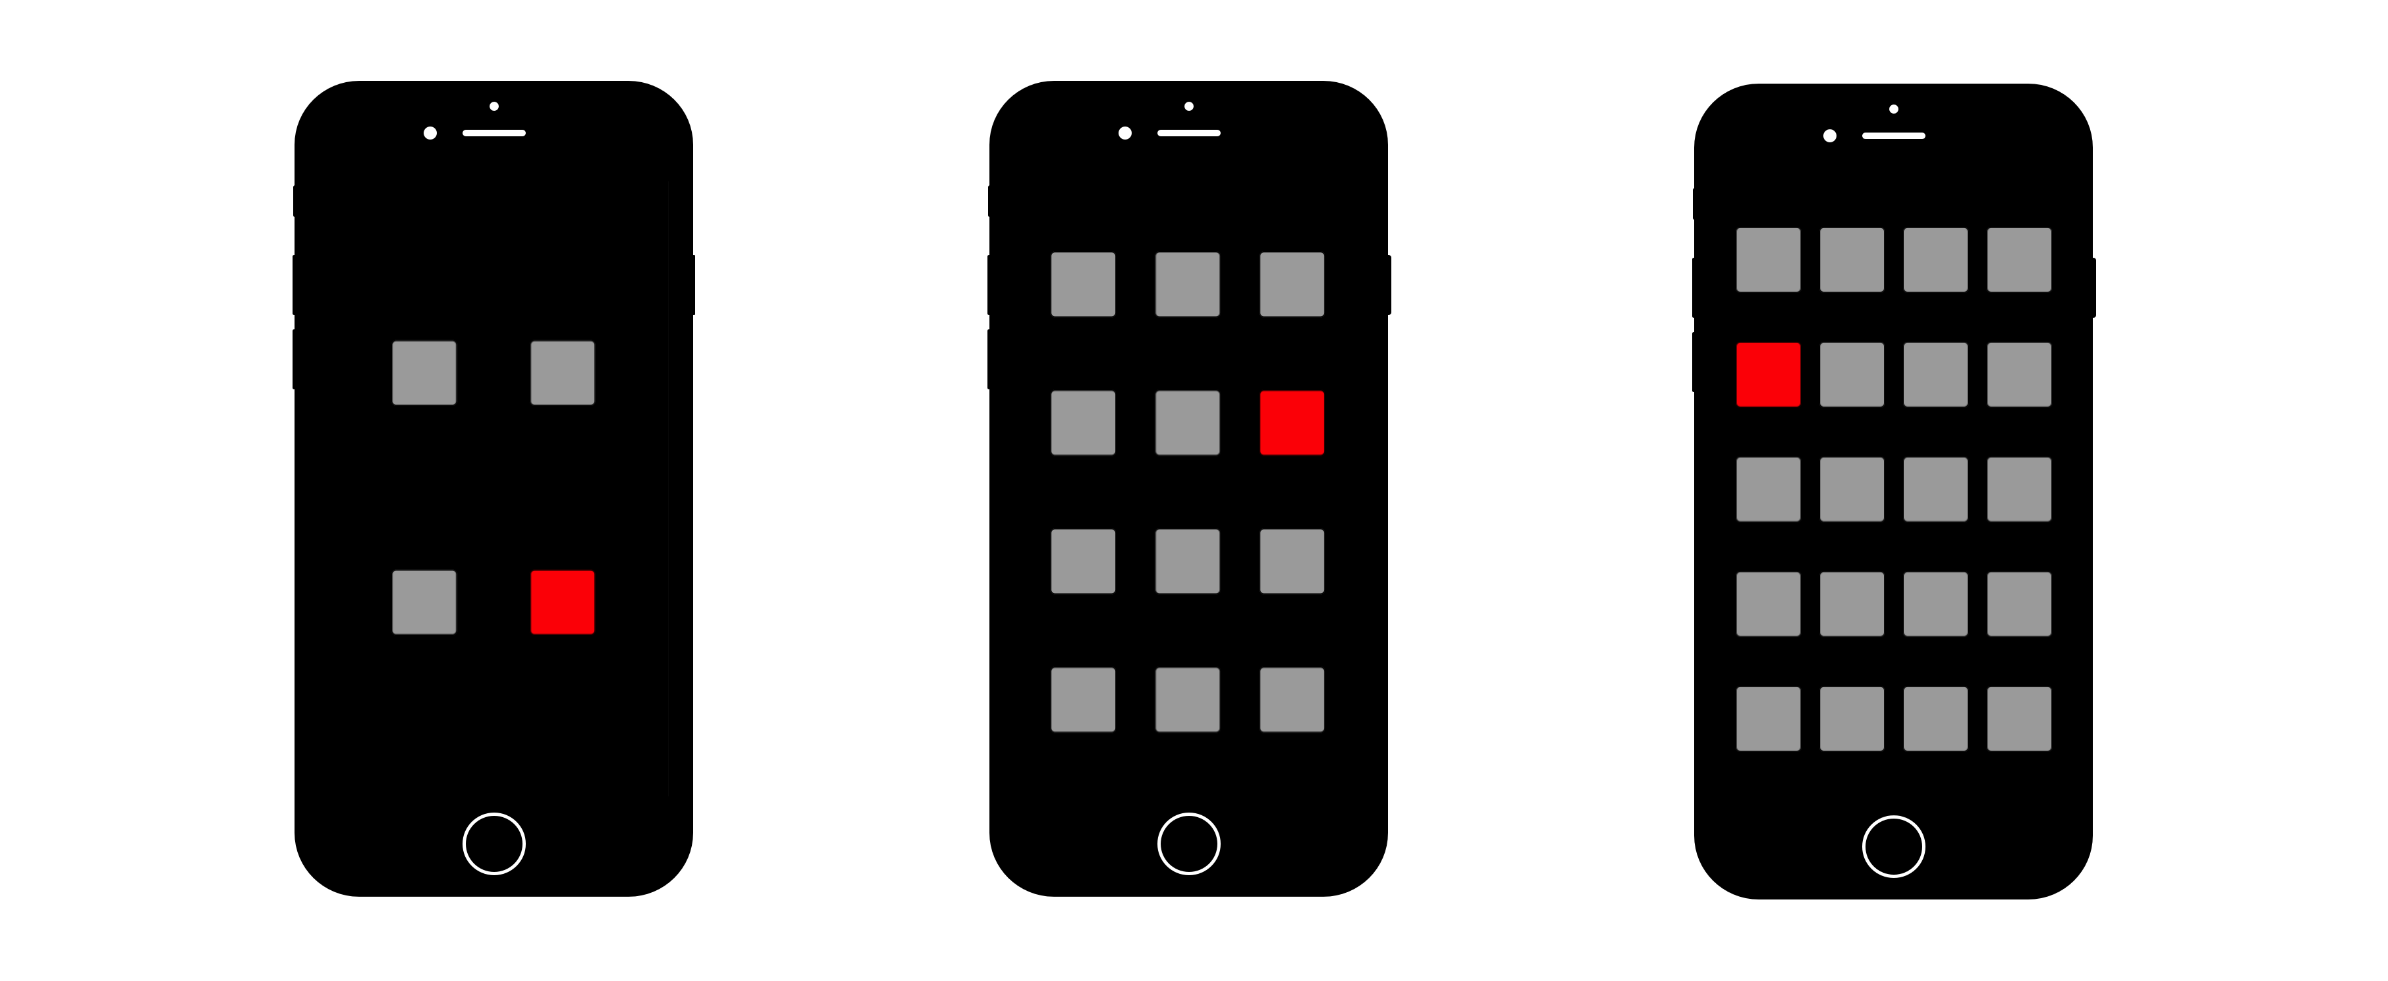
\includegraphics[width=0.8\textwidth]{grids_iphone.png}
  \caption{Grid sizes of Grid. }
\end{figure}

For the user to be able to enter the taps into the device the app provides a screen with buttons aligned in grip structures.\\

The positions of the buttons are calculated based on the configuration that is set. Here, the amount of buttons in height and width can be adjusted. \\
% Maybe a table
% \begin{itemize}
% \item 2 x 2
% \item 4 x 3
% \item 4 x 5
% \end{itemize}

% \begin{center}
%     \begin{tabular}{ | l | l | l | }
%     \hline
%     \# & height & width \\ \hline
%     1 & 2 & 2 \\
%     2 & 4 & 3 \\
%     3 & 4 & 5 \\
%     \hline
%     \end{tabular}
% \end{center}

The source code of the of the question view is to be found in \texttt{GridViewController.swift}.


\subsubsection{Questions}
To obtain more information on the taps provided in the tap input view, the application provides views for the user to answer several questions concerning input modalities, body posture and mood.
After the tap input screen, the questions are displayed providing multiple answer choices. In addition, the application provides a pictogram for each answer option.

\begin{figure}[h!]
  \centering
  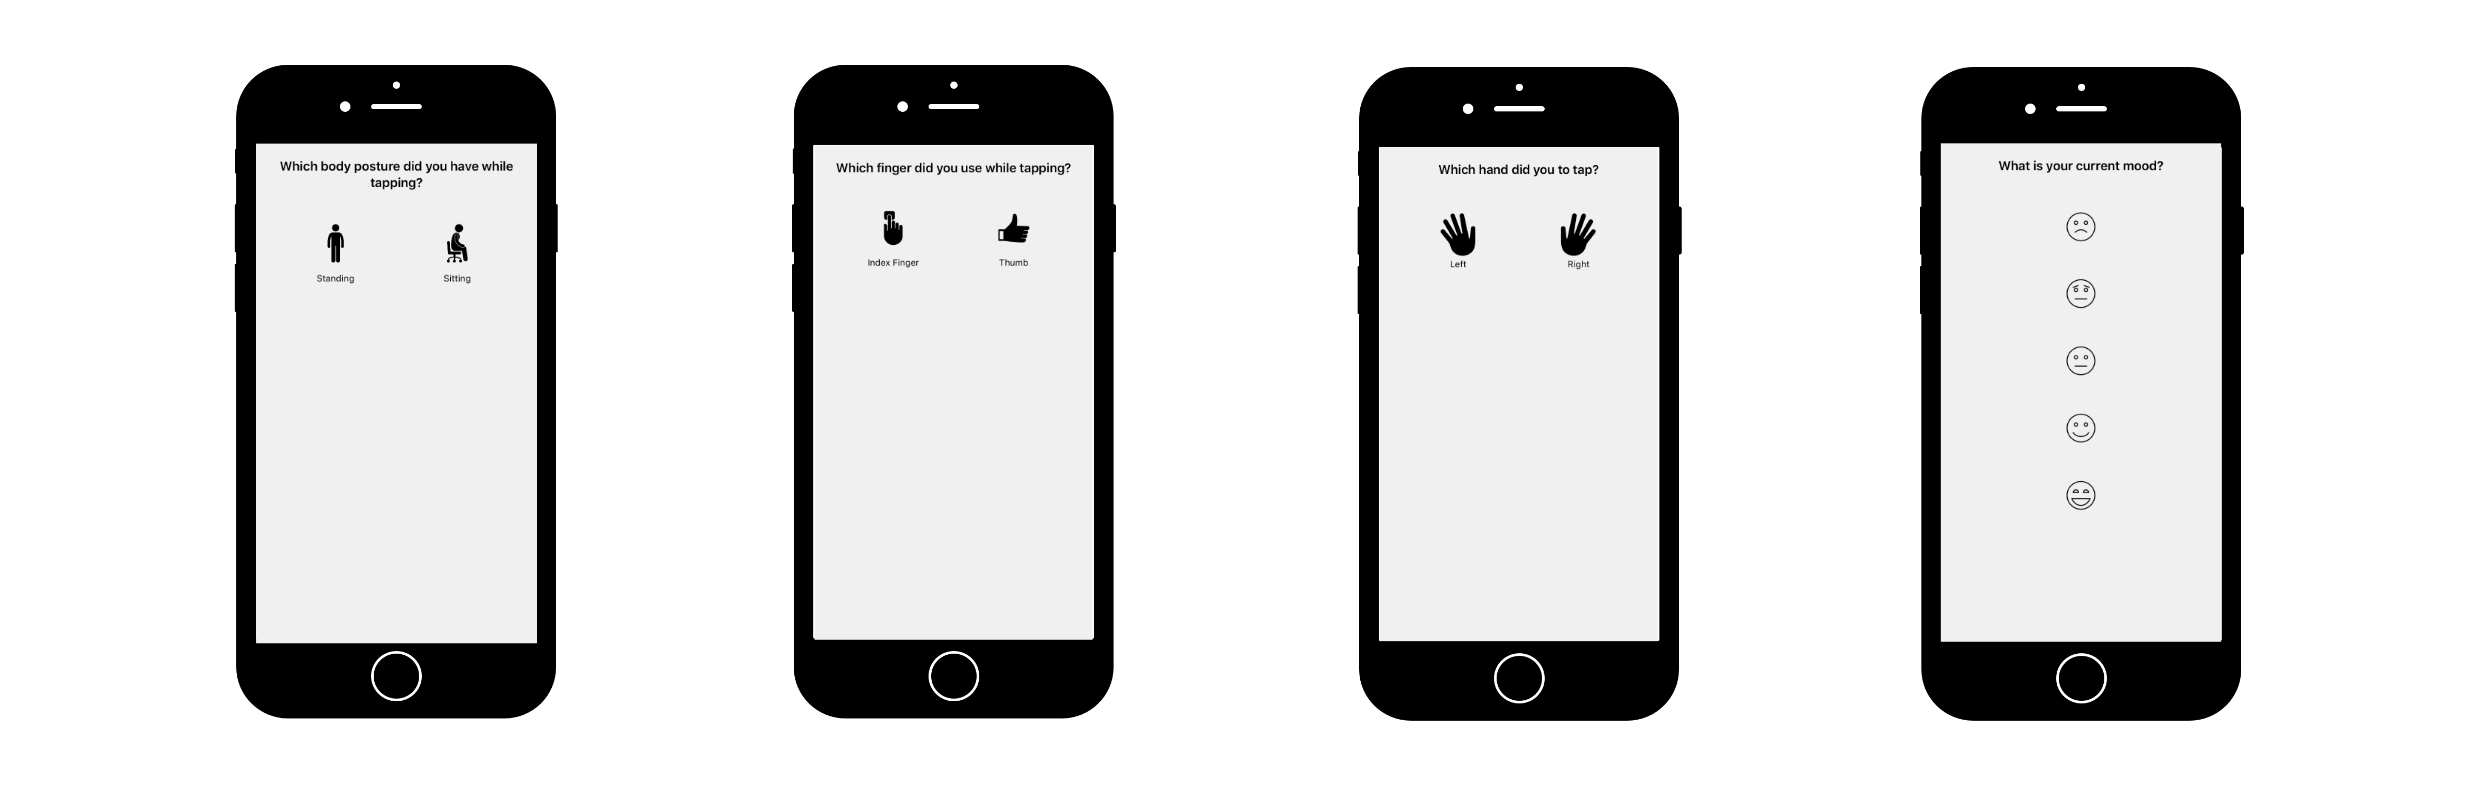
\includegraphics[width=1\textwidth]{questions_iphone.png}
  \caption{The figure displays question views with icons as answer possibilities.}
\end{figure}

Each view is generically set based on the questions and answer possibilities. Once the user taps on an icon the view transitions to the next question view.\\ 

The source code of the of the question view is to be found in \texttt{QuestionViewController.swift}.

\subsubsection{Upload}
After all taps and additional information is gathered, we show a view that the application is uploading the data to the server-side application. 

\subsection{Smartphone Sensors}
Modern smartphones come with a variety of different sensors offering valuable services to it's users and enhancing many applications. The newest Apple iPhone to date, the iPhone 7, has a fingerprint sensor, a barometer, a three-axis gyroscope and accelerometer (MEMS), a proximity sensor and an ambient light sensor attached to it's main-board \cite{iphone7techspecs}. As we are going to predict finger taps on the iPhone screen, the only sensors that are effected by the force of the tap are the gyroscope and the accelerometer. Therefore, these will be outlined in the following sections.

\subsubsection{Accelerometer}

The accelerometer is a sensor module that measures the acceleration it encounters by either movement or gravity \cite{sensorsstudy}. However, the acceleration caused by movement, the so-called inertial acceleration and the gravitational acceleration can not be distinguished by the sensor. This is due to Einstein's equivalence principal stating that the effects of gravity on an object are indistinguishable from the acceleration of the object's reference frame \cite{doi:10.1021/ed014p49.2}. \\

\begin{figure}[h!]
  \centering
  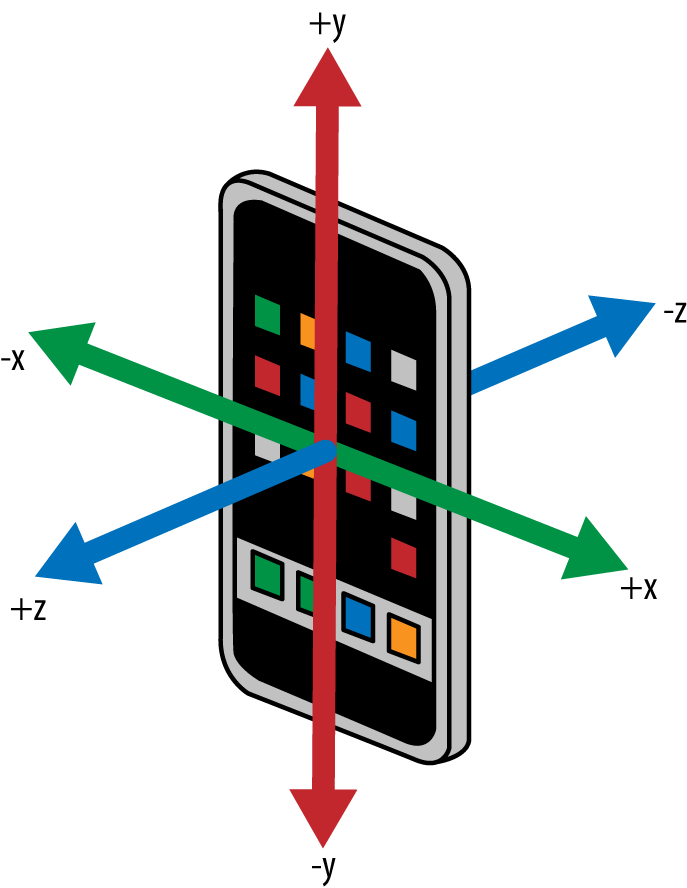
\includegraphics[width=0.35\textwidth]{iphone-acc.png}
  \caption{Apple iPhone with the corresponding axes of the accelerometer.}
\end{figure}

When the position of the device is fixed, as for example when it is placed on a table the accelerometer values would yield $a = \{ a_x = 0, a_y = 0, a_z = -1\}$. This feature make it suitable for detecting device screen rotations. As the device flips from landscape to portrait orientation, the gravity is sensed by a different set of accelerometer axis \cite{sensorsstudy}.\\

The values of the acceleration are quantified in the SI unit metres per second per second ($m/s^2$). However, in engineering the acceleration is typically expressed in terms of the standard gravity ($g$).

\subsubsection{Gyroscope}

As the accelerometer is suitable for detecting orientations, it lacks the ability to detect spin or more precise rotation movements. These spin movements are detected by the gyroscope sensor which is responsible for detecting and maintaining orientation \cite{sensorsstudy}. \\

A mechanical gyroscope typically composes of a spinning wheel which is set within three so-called gimbals. These gimbals enable the spinning wheel to be set in any orientation. Although the orientation does not remain fixed when the device is rotated, it changes in response to an external torque much lesser and in a different direction than it would be without the large angular momentum associated with it. Each gimbals translates to one of the three gyroscope outputs, namely \textit{pitch}, \textit{roll} and \textit{jaw} (See \cite{wiki:Gyroscope}). \\

The gyroscope sensor within the MEMS\footnote{Microelectromechanical systems}, the chip deployed in the iPhone, is between 1 to 100 micrometers of size. When the gyroscope is rotated, a small resonating mass is shifted as the angular velocity changes. This movement is converted into very low-current electrical signals that can be amplified and read by a host system. \\

The values of the gyroscope are quantified in as rotations per seconds (RPS) or as degrees per second ($\deg/s$).

\subsubsection{Accessing sensor values}
% Apple offers api for accessing these values.
In order to access gyroscope and accelerometer Apple provides a high level API\footnote{An Application Program Interface is a set of rules and subroutines provided by an application system for the developer to use. Here is a link to the Core Motion API Documentation: \url{https://developer.apple.com/documentation/coremotion/} } for accessing the device's sensors: \texttt{Core Motion}. Core Motion reports motion and environmental related data from sensors including accelerometers, gyroscopes, pedometers, magnetometers, and barometers in easy to use manner. \\

Sensor values can either be accessed as proceeded version including aggregations of the values and a raw version. For TapSensing, we make sure to record the raw values to avoid any form of bias. The update interval can be configures at ranges from $10$Hz - $100$Hz. Higher update-rates are possible but are not ensured to be processed in real-time by the device. For TapSensing, the update rate is configured with the highest (safe) value possible. This ensures that tap patterns are captured with an accurate resolution to make a later classification easier. The figure below is a code snipping depicting how sensor values are retrieved in the TapSensing application.

\begin{figure}[thp]
\centering
\begin{minipage}{0.7\textwidth}

\begin{minted}{swift}
let UPDATE_INTERVAL = 0.01
let motionManager = CMMotionManager()

// Set the update interval on both sensors
motionManager.gyroUpdateInterval = UPDATE_INTERVAL
motionManager.accelerometerUpdateInterval = UPDATE_INTERVAL

// Start reading the sensor values
motionManager.startAccelerometerUpdates()
motionManager.startGyroUpdates()

// Pass in a function to handle sensor update values,
// which arrive in the update interval rate.
motionManager.startAccelerometerUpdates(to: .bg) {
    (data: CMAccelerometerData?, error: Error?) in
    // handle incoming data
    ...
}
motionManager.startGyroUpdates(to: .bg) {
    (data: CMGyroData?, error: Error?) in
    // handle incoming data
    ...
}
\end{minted}
\end{minipage}
\caption{Swift code snippet displaying how to access sensor values with Core Motion.}
\label{test}
\end{figure}

\textbf{Interoperability}
-JSON
\textbf{Scalability}
-Machine

\section{Backend application}
\subsection{General requirements}
\subsubsection{Security}
\subsubsection{Consistency}
\subsection{}
\subsection{Data model}
\subsection{User management \& Security}
\subsection{Ensuring consistency}